\newpage
\section{State of the art}\label{s:SOTA}
I dette afsnit har vi forsøgt at finde en bred vifte af forskellige løsninger, der kan løse et eller flere problemer i forbindelse med indkøb og madlavning, omhandlende indkøbslister, tilbud og opskrifter.

Der vil blive kigget på web services og applikationer, der har til formål at løse nogle af de samme problemer, der berører vores emne.
Løsningerne, der er præsenteret i dette afsnit, forsøger at afhjælpe de problemer beskrevet af de adspurgte i interviewene i \myref{section:interview1}.

\subsection{eTilbudsavis}
eTilbudsavis er en online service, der kan findes på deres hjemmeside\footnote{\underline{www.etilbudsavis.dk}} og deres app på forskellige mobilplatforme.
eTilbudsavis er en online avis med en høj funktionalitet og en nem brugergrænseflade.
Der kan på siden oprettes et login, således kan der findes tilbage til ændringer på et senere tidspunkt eller andre enheder.
eTilbudsavis har tre mærkbare funktioner, som brugeren har adgang til, hvilket er tilbudsaviser, ønske- og indkøbslister og tilbud.

Tilbudsavis-funktionen, som kan ses på \myref{ss:eTilbudsavis}, indeholder også den mulighed at sætte en præference på, hvor stor en radius man vil lede i efter butikkers tilbudsaviser.
Under hver avis, som det ses på figuren, er der også angivet afstand i meter fra ens aktuelle placering.
Der kan vælges imellem alle aviser, som er tilgængelige online og inden for den valgte radius.
Aviserne bliver opdateret løbende, så når der er en ny tilgængelig, bliver den gamle fjernet.
Inde i aviserne kan man trykke på et tilbud, og dette tilføjes til en liste.

\begin{wrapfigure}{o}{0.68\textwidth}
\vspace{-20pt}
	\begin{center}
		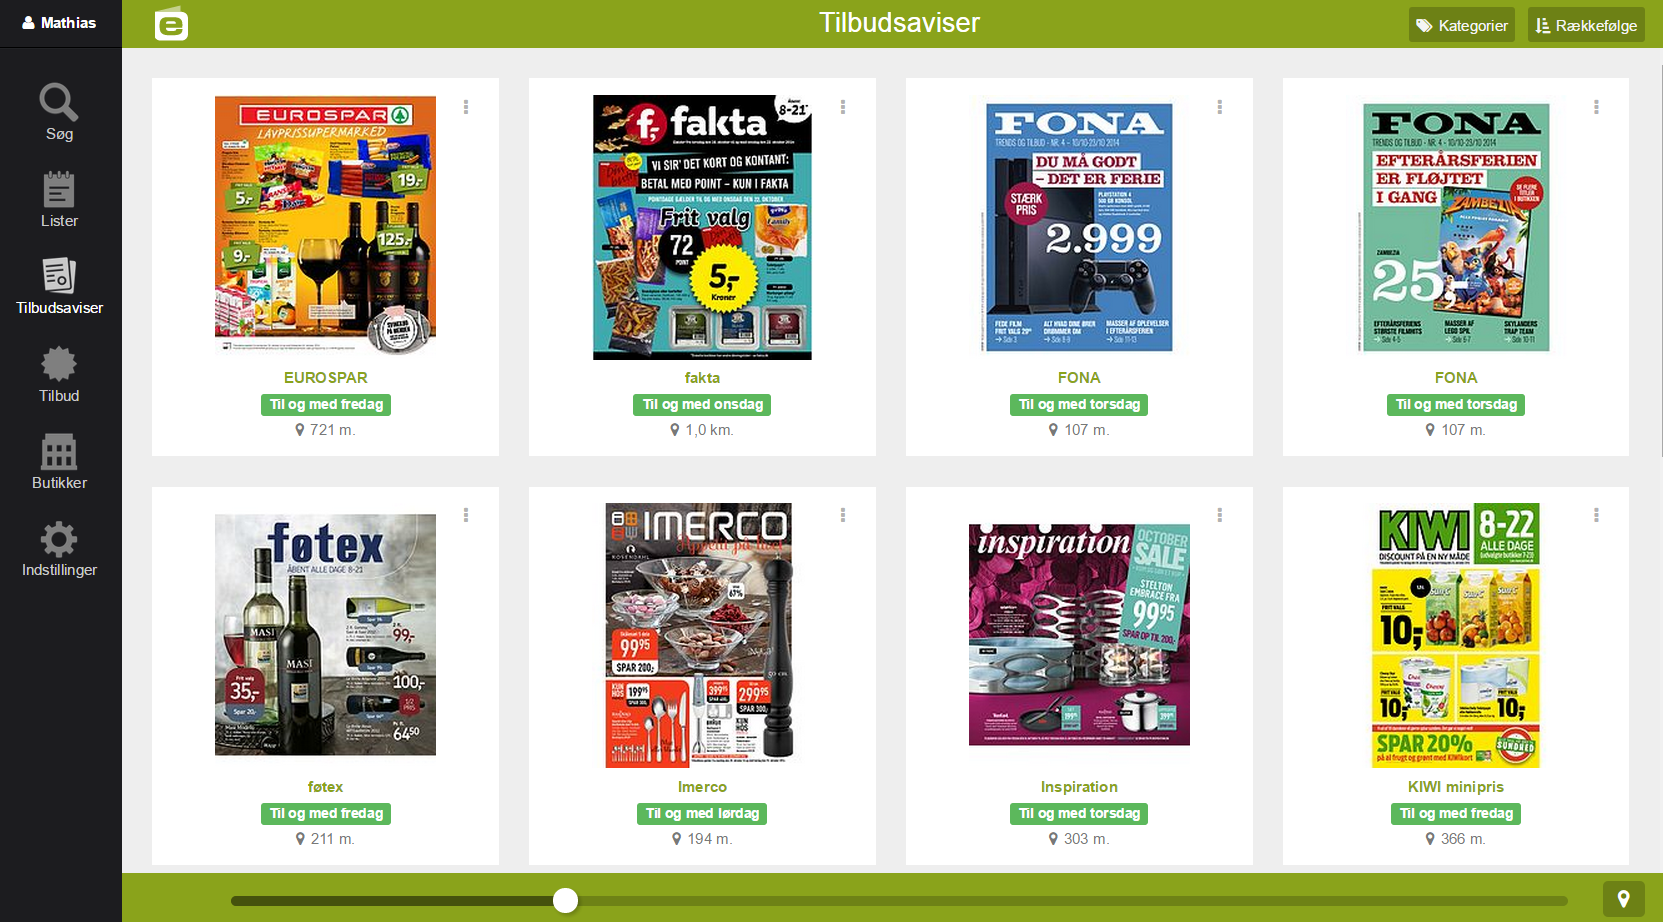
\includegraphics[width=0.66\textwidth]{images/Images/eTilbudsavis.PNG}
	\end{center}
	\vspace{-20pt}
	\caption{Tilbudsaviser på eTilbudsavis.dk}\label{ss:eTilbudsavis}
	\vspace{-20pt}
\end{wrapfigure}

Der er mulighed for at tilføje varer til to lister, en indkøbsliste og/eller en ønskeliste.
Når en vare er valgt, bliver den tilføjet til den valgte liste.
Listen indeholder navn, butik, pris og den valgte mængde, for varen.
Der kan, foruden det at vælge varer fra tilbudsaviserne, nemt skrives generiske varer på listen. Varen på listen kan da krydses af for at kunne holde styr på, hvad der er blevet købt.

Hvis der ikke ønskes at skulle bladre igennem tilbudsaviser, er der den mulighed at få vist en hel side kun med tilbud.
Alle aktuelle tilbud fra aviserne, er da vist, som elementer med navn, beskrivelse, pris, butik og afstand. 
Disse tilbud kan på samme måde nemt tilføjes til listerne.

\subsection{Tilbudsugen}
Tilbudsugen minder på mange måder om eTilbudsavis, og kan findes på deres hjemmeside\footnote{\underline{www.tilbudsugen.dk}}.
Den har samtlige dagligvareaviser, samt flere inden for bl.a. byggemarkeder, og autoudstyr.
De giver et nemt overblik over diverse aviser, og man kan hurtigt og nemt læse dem på nettet.
Der er desuden mulighed for at lave præferencer som ved eTilbudsavis, her kan man bl.a. vælge økologi eller nøglehulsmærket.
Når man tilføjer en vare til indkøbslisten, søger den automatisk efter tilbud på den valgte vare.
Man bliver bedt om at vælge et specifikt tilbud, og netop dette tilbud bliver tilføjet til indkøbslisten med pris, butik, udløbsdato, mængde og et billede af varen.
Man kan, som på eTilbudsavis, også trykke på en vare direkte i avisen for at tilføje den til sin liste.
Hvis man vil dele sin indkøbsliste, er det også en mulighed vha. en delekode som man kan give til en anden bruger - de kan på denne måde også se listen.
Funktionerne findes på hjemmesiden, men det er ikke altid de virker.
For eksempel hvis man tilføjer noget uden at angive et antal, og du så prøver at dele listen med en, vil det ikke være at finde på listen.
Desuden kan man ikke ændre på antallet af en vare, du allerede har sat på din indkøbsliste.
For at opnå dette, skal man slette varen, og tilføje den igen med det nye antal.
De har desuden også en smartphone app, men vores test af systemet indikerer, at denne ofte crasher, når man benytter sig af deres indkøbsliste, men fungerer tilgengæld fint, hvis man blot vil se på ugens tilbud i aviserne.

Tilbudsugen er et lidt dårligere alternativt til eTilbudsavis, da der er problemer med delbarheden af indkøbslisterne, samt den app, der er stillet til rådighed, ikke er stabil.
Derimod er den nem at navigere, siden er brugervenlig og ser overskuelig ud.

\subsection{Smartphone Apps udgivet af butikker}
På \myref{tbl-smartphone} ses der nogle butikskæder, som har udviklet android apps, samt hvilke funktionaliteter disse apps har.
For at skabe et overblik, er der udvalgt features, og disse er blevet opsat i et skema for overskuelighedens skyld.
\begin{table}[H]
	\centering
		\colorlet{shadecolor}{gray!40}
    	\rowcolors{1}{white}{shadecolor}
	    \begin{tabular}{l|lllllllllll}
	    %Table: http://bit.ly/1tD6EI6
	   	%Funktionalitet & Tilbudsavis & Indkøbsliste & Opskrifter & Varescan & Find butik & Budget & Madplan & Rabatkupon/fordelsordning & Deling af indkøbslister & Rating på Play & Senest opdateret \\ \hline
	     & \rot{Tilbudsavis} & \rot{Indkøbsliste} & \rot{Opskrifter} & \rot{Varescan} & \rot{Find butik } & \rot{Budget} & \rot{Madplan} & \rot{Rabatkupon} & \rot{Deling} & \rot{Play rating} & \rot{Senest} \rot{opdateret} \\ \hline
	   	Føtex                       & \cmark   & \cmark    & \cmark  & \cmark   & \cmark  & ~      & ~       & ~          & ~                       & 3.4 (354)      & 2014-07-24       \\
	    SPAR                        & \cmark   & \cmark    & \cmark  & ~        & \cmark  & \cmark & ~       & ~          & ~                       & 2.8 (64)       & 2014-05-15       \\
	    Fakta                       & \cmark   & \cmark    & \cmark  & ~        & \cmark  & ~      & \cmark        & \cmark     & \cmark               & 3.1 (454)      & 2014-08-02       \\
	    FaktaQ                      & \cmark   & ~         & \cmark  & ~        & \cmark  & ~      & ~       & ~          & ~                       & 4.4 (7)        & 2014-03-11       \\
	    REMA 1000                   & \cmark   & \cmark    & \cmark  & ~        & \cmark  & ~      & ~       & ~          & ~                       & 3.5 (674)      & 2014-04-16       \\
	    SuperBrugsen                & \cmark   & \cmark    & \cmark  & ~        & \cmark  & ~      & ~       & ~          & ~                       & 3.8 (987)      & 2014-06-30       \\
	    Kvickly                     & \cmark   & \cmark    & \cmark  & ~        & \cmark  & ~      & ~       & ~          & ~                       & 3.7 (632)      & 2014-07-20       \\
	    \end{tabular}
	    \caption{Nogle butikskæder med smartphone apps samt deres funktionaliteter.}\label{tbl-smartphone}
	\end{table}
Vi har valgt at beskrive en af disse apps nærmere, og valget faldt på Faktas app, MitFakta, da denne bliver opdateret og har flest funktioner.
\subsubsection{Faktas Android App}

\begin{wrapfigure}{o}{0.4\textwidth}
\vspace{-20pt}
	\begin{center}
		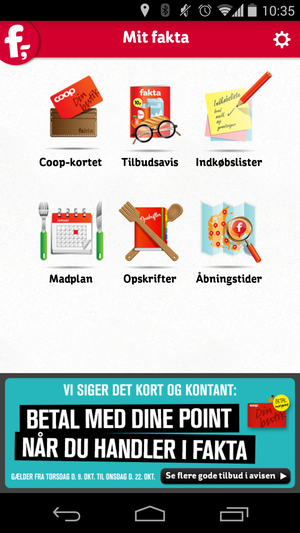
\includegraphics[width=0.38\textwidth]{images/Images/MitFakta.png}
	\end{center}
	\vspace{-20pt}
	\caption{MitFakta}
	\vspace{-20pt}
	\label{ss:MitFakta}
\end{wrapfigure}

Faktas android app er som helhed overskuelig.
Efter åbning af appen kan man vælge mellem seks menupunkter eller ændre sine indstillinger, disse kan ses på \myref{ss:MitFakta}.
Første menupunkt omhandler ``Coop-kortet'' og giver brugeren mulighed for at indtaste sine medlemsinfomationer, da disse giver særlige tilbud.
Andet menupunkt er deres tilbudsavis, hvilket er en digital udgave af den fysiske tilbudsavis.
Dog kan man fra den også tilføje varer til sin indkøbsliste, eller se varerne i et gitterformat.
Tredje menupunkt er ``indkøbsliste''; her kan man have flere personlige og/eller delte indkøbslister.
Det er også her, deres Facebook integration kommer i spil, som tillader nem deling af indkøbslister med brugerens Facebook venner.
Fjerde menupunkt er en madplan, hvori man kan planlægge sin egen madplan, eller se Faktas anbefalinger til en ``under 20 kr pr. person pr. aften''-løsning.
Femte menupunkt er deres opskrifter.
Her findes der et stort antal af opskrifter, disse kan tilføjes direkte til ens madplan eller indkøbslister (både personlige og delte).
Sjette menupunkt hedder ``Åbningstider'', hvor brugeren kan finde Faktas butikker samt deres forskellige åbningstider.

Appen virker rigtig godt, der er ingen blindgyder, og derfor er den meget nem at navigere rundt i. 
Der er lagt fokus på den sociale del, da der kan deles med venner på facebook, hvilket simplificerer delingen af indkøbslister. 
Den eneste ulempe, der er ved denne app, er, at den kun er egnet til vare fra Fakta, og derfor sætter en del restriktioner på sig selv.

\subsection{Tøm køleskabet} 
Der findes talrige tjenester, der tilbyder ``at tømme dit køleskab''.
Mere specifikt tilbyder de en service, hvor du som bruger, angiver hvilke varer dit køleskab pt. indeholder, samt hvilke andre ingredienser du har til rådighed.
Derefter får du så præsenteret en række forskellige opskrifter, der kan laves ud fra dine tilgængelige ingredienser.
De fleste af tjenesterne (herunder dem vi her har undersøgt) viser også opskrifter, som indeholder yderligere ingredienser.
Dette betyder, at man som bruger ikke bliver fritaget fra at handle ind, hvis man mangler nogle ingredienser til lige netop den opskrift, man vælger at udføre.
Tjenesten \textit{MyFridgeFood} \footnote{\underline{www.myfridgefood.com}} tilbyder at oprette en indkøbsliste ud fra netop disse manglende ingredienser, hvilket kan lade sig gøre blandt andet fordi, alle opskrifter er interne på \textit{MyFridgeFood}.
I modsætning til dette er der \textit{Supercook} \footnote{\underline{www.supercook.com}}, som linker til eksterne opskrifter, og ikke tilbyder at generere en indkøbsliste.
Umiddelbart anbefales opskrifter ikke ud fra den enkelte brugers smag og madvaner, men udelukkende på baggrund af, hvad man ``har i køleskabet''.
Grundet dette virker tjenesterne mere som simple filtreringer af databaseopslag, end egentlige anbefalinger, der tager højde for brugerens smag og præferencer indenfor den gastronomiske verden.

Som vi har set, findes der alternativer til den klassiske indkøbstur, der er dog ingen af disse, der formår at løse alle problemerne.
Ved alle løsningerne opstår også nye ulemper og problemstillinger i forhold til almindeligt indkøb.
Alt taget i betragtning vil det komme meget an på nuværende vaner og familiestrukturen, om disse muligheder vil være en god løsning for en given familie.
